\chapter{花、果实与种子}\label{ch:g3:flowers-fruits-seeds}

四月，樱桃树开满白色的花；六月，
枝头挂满了樱桃。花去哪儿了——
\omterm{prop:g3:flowers-fruits-seeds:transform}{果实}又是从哪里来的？答案是\omterm{def:g1:living-or-not:living}{生物}界最美妙的
过程之一：花并没有消失，
而是\emph{变成了}\omterm{prop:g3:flowers-fruits-seeds:transform}{果实}。

\section{观察花的内部}

\begin{definition}[花的组成部分]\label{def:g3:flowers-fruits-seeds:parts}
\emph{花}\index{花}是\omterm{def:g1:plants-around-us:plant}{植物}中
将来能产生\omterm{def:g2:from-seed-to-plant:seed}{种子}的部分。从外向内看：
\begin{enumerate}
  \item \emph{花瓣}\index{花瓣}，颜色鲜艳、带有香味，
        能吸引来访的\omterm{prop:g3:sorting-living-things:groups}{昆虫}；
  \item \emph{雄蕊}\index{雄蕊}，细长的柄，柄上撒满
        \emph{花粉}\index{花粉}，细细的黄色粉末；
  \item 位于花的正中央的\emph{雌蕊}\index{雌蕊}，
        形状像一个小瓶子，瓶子深处藏着花的
        未来的\omterm{def:g2:from-seed-to-plant:seed}{种子}。
\end{enumerate}
\end{definition}

\begin{omfigure}
\begin{tikzpicture}
  \node[anchor=south west, inner sep=0] (img) at (0,0)
    {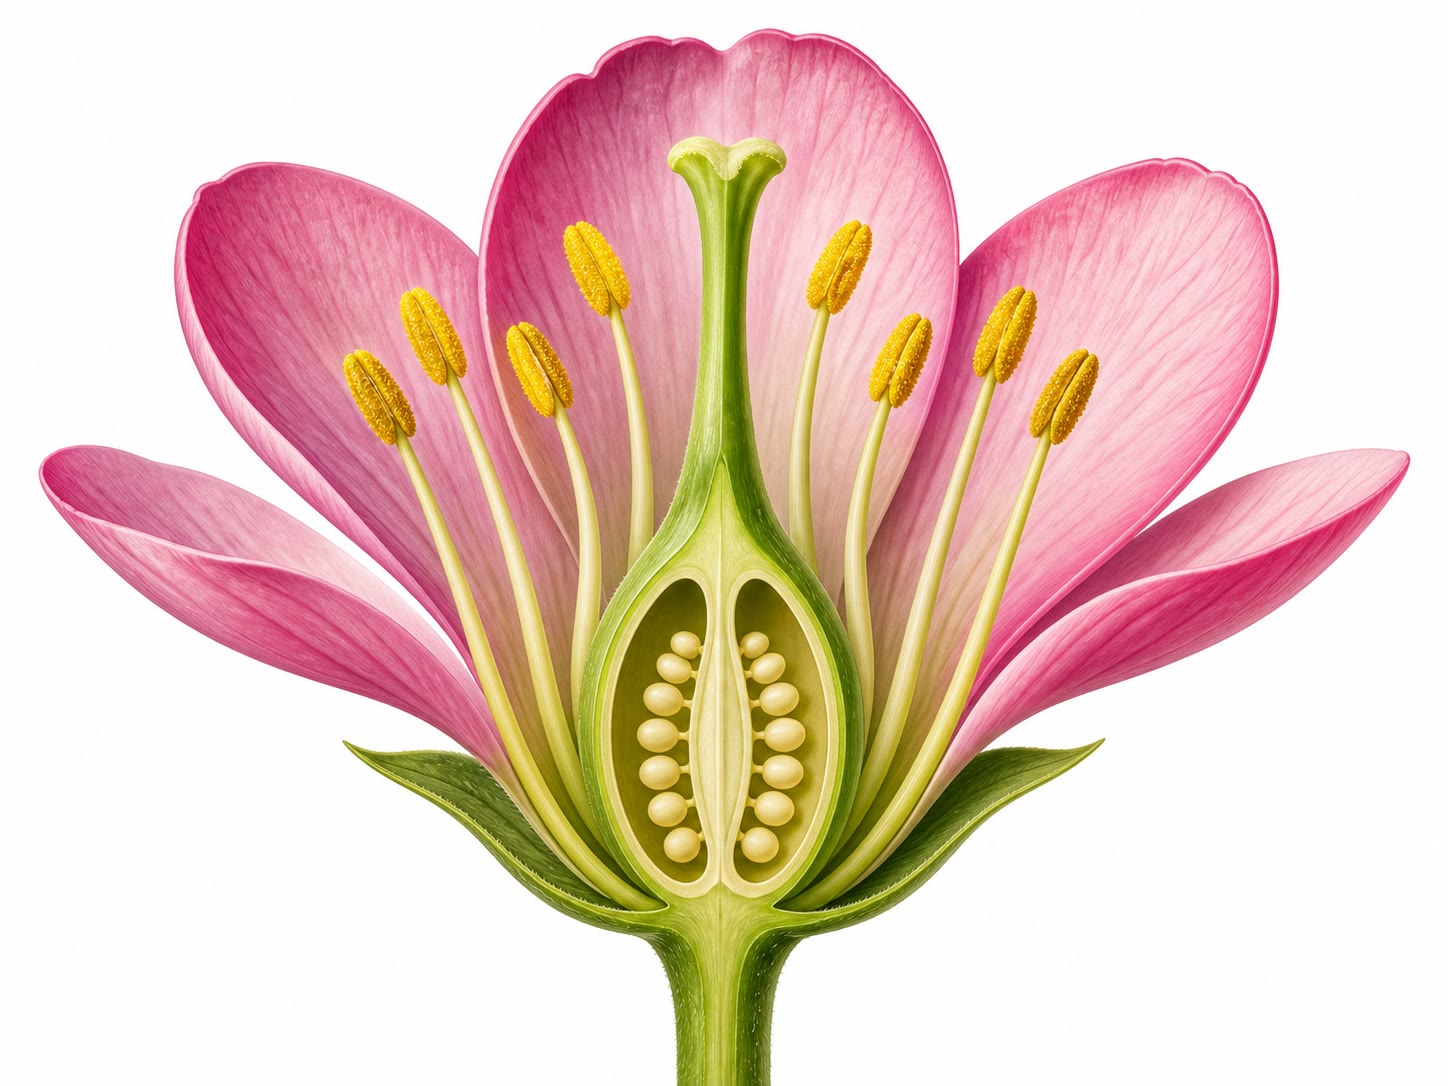
\includegraphics[width=0.6\linewidth]{images/book1/ai/fig-flower-cutaway.jpg}};
  \begin{scope}[x={(img.south east)}, y={(img.north west)},
      every node/.style={font=\small}]
    \draw[omDef, thick] (0.82,0.80) -- (0.93,0.90) node[above] {花瓣};
    \draw[omDef, thick] (0.72,0.68) -- (1.03,0.66)
      node[right, align=left] {雄蕊，\\ 带有花粉};
    \draw[omDef, thick] (0.56,0.36) -- (1.03,0.34)
      node[right, align=left] {雌蕊：\\ 内有未来的种子};
    \draw[omDef, thick] (0.505,0.05) -- (0.66,0.04) node[right] {茎};
  \end{scope}
\end{tikzpicture}

{\small 花从中间切开后的内部：周围是\omterm{def:g3:flowers-fruits-seeds:parts}{花瓣}，带有\omterm{def:g3:flowers-fruits-seeds:parts}{花粉}的\omterm{def:g3:flowers-fruits-seeds:parts}{雄蕊}，
正中央是\omterm{def:g3:flowers-fruits-seeds:parts}{雌蕊}，\omterm{def:g3:flowers-fruits-seeds:parts}{雌蕊}内藏着未来的\omterm{def:g2:from-seed-to-plant:seed}{种子}。}
\end{omfigure}

\begin{example}[解剖一朵郁金香]\label{ex:g3:flowers-fruits-seeds:tulip}
轻轻打开一朵快要凋谢的郁金香，一片\omterm{def:g3:flowers-fruits-seeds:parts}{花瓣}一片\omterm{def:g3:flowers-fruits-seeds:parts}{花瓣}地掀开。里面立着
\omterm{def:g3:flowers-fruits-seeds:parts}{雄蕊}——用手指碰一碰，手指上就会沾上黄色的\omterm{def:g3:flowers-fruits-seeds:parts}{花粉}
，中间是肥厚的绿色\omterm{def:g3:flowers-fruits-seeds:parts}{雌蕊}。把\omterm{def:g3:flowers-fruits-seeds:parts}{雌蕊}横着切开
（请大人帮忙下刀），就能看到一排排
细小、浅色的未来\omterm{def:g2:from-seed-to-plant:seed}{种子}。
\end{example}

\section{从花到果实}

\begin{proposition}[传粉，然后转化]\label{prop:g3:flowers-fruits-seeds:transform}
要使转化开始，\omterm{def:g3:flowers-fruits-seeds:parts}{花粉}必须到达\omterm{def:g3:flowers-fruits-seeds:parts}{雌蕊}——
这一步叫作\emph{传粉}\index{传粉}。蜜蜂和
其他\omterm{prop:g3:sorting-living-things:groups}{昆虫}承担了大部分搬运工作，它们
在一朵接一朵的花上吸食花蜜，身上沾满\omterm{def:g3:flowers-fruits-seeds:parts}{花粉}；风也起了一些作用。
传粉之后：
\begin{itemize}
  \item \omterm{def:g3:flowers-fruits-seeds:parts}{花瓣}和\omterm{def:g3:flowers-fruits-seeds:parts}{雄蕊}完成了任务，便凋谢、脱落；
  \item \omterm{def:g3:flowers-fruits-seeds:parts}{雌蕊}膨大，变成
        \emph{果实}\index{果实}；
  \item \omterm{def:g3:flowers-fruits-seeds:parts}{雌蕊}内将来的\omterm{def:g2:from-seed-to-plant:seed}{种子}，变成
        \emph{种子}\index{种子}。
\end{itemize}
\omterm{prop:g3:flowers-fruits-seeds:transform}{果实}是转化后的\omterm{def:g3:flowers-fruits-seeds:parts}{雌蕊}，每一个真正的\omterm{prop:g3:flowers-fruits-seeds:transform}{果实}
都含有\omterm{def:g2:from-seed-to-plant:seed}{种子}。
\end{proposition}
\admitted

\begin{example}[观察一颗樱桃的形成]\label{ex:g3:flowers-fruits-seeds:cherry}
跟踪一朵樱桃花的变化。四月：白色的\omterm{def:g3:flowers-fruits-seeds:parts}{花瓣}，蜜蜂
嗡嗡地飞来。五月：\omterm{def:g3:flowers-fruits-seeds:parts}{花瓣}像雪花一样飘落；每朵花原来所在的地方，
长出一个小小的绿色圆球——那是膨大的\omterm{def:g3:flowers-fruits-seeds:parts}{雌蕊}。六月：圆球长成了红色、
甜甜的樱桃，里面有一颗核（也就是\omterm{def:g2:from-seed-to-plant:seed}{种子}）。花并没有掉落，
掉落的只是\omterm{def:g3:flowers-fruits-seeds:parts}{花瓣}。
\end{example}

\begin{remark}[没有蜜蜂，就没有樱桃]\label{rem:g3:flowers-fruits-seeds:bees}
樱桃种植者欢迎养蜂人把蜂箱搬进果园——
没有\omterm{prop:g3:sorting-living-things:groups}{昆虫}来访，大多数花都得不到授粉，
只会凋落，永远无法变成\omterm{prop:g3:flowers-fruits-seeds:transform}{果实}。蜜蜂并不是在从花上窃取，
而是与花互相帮助：花为蜜蜂提供花蜜，
蜜蜂则为\omterm{def:g1:plants-around-us:plant}{植物}传递\omterm{def:g3:flowers-fruits-seeds:parts}{花粉}。
\end{remark}

\begin{omfigure}
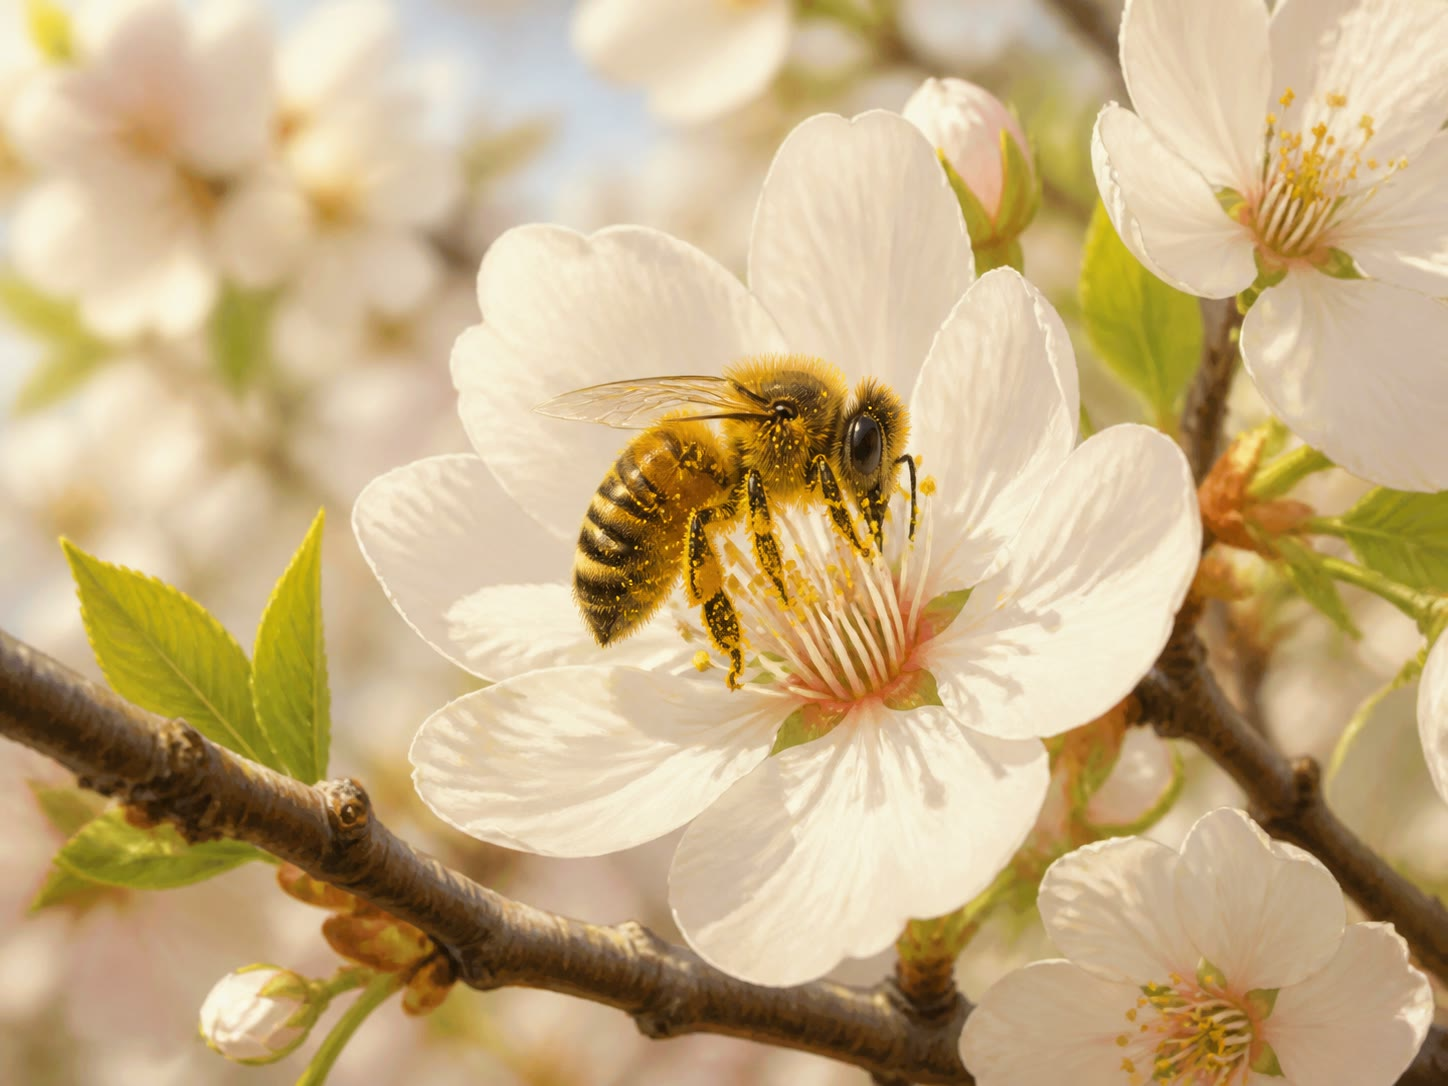
\includegraphics[width=0.58\linewidth]{images/book1/ai/g3-flowers-bee.jpg}

{\small 正在传粉：一只蜜蜂钻进樱桃花深处，
身上沾满将要带给下一朵花的\omterm{def:g3:flowers-fruits-seeds:parts}{花粉}。}
\end{omfigure}

\section{是果实，还是不是果实？}

\begin{method}[种子检验法]\label{met:g3:flowers-fruits-seeds:test}
要判断菜市场上买来的某样东西，
在生物学意义上是否属于\omterm{prop:g3:flowers-fruits-seeds:transform}{果实}：
\begin{enumerate}
  \item 把它切开；
  \item 寻找\omterm{def:g2:from-seed-to-plant:seed}{种子}（或者一颗核，核
        就是外面包着硬壳的\omterm{def:g2:from-seed-to-plant:seed}{种子}）；
  \item 内有\omterm{def:g2:from-seed-to-plant:seed}{种子}——它由花的\omterm{def:g3:flowers-fruits-seeds:parts}{雌蕊}发育而来，是\omterm{prop:g3:flowers-fruits-seeds:transform}{果实}。
        找不到任何\omterm{def:g2:from-seed-to-plant:seed}{种子}——它是\omterm{def:g1:plants-around-us:plant}{植物}的其他部分：
        根、茎或叶。
\end{enumerate}
\end{method}

\begin{example}[菜市场里的意外]\label{ex:g3:flowers-fruits-seeds:surprise}
用\omterm{def:g2:from-seed-to-plant:seed}{种子}检验法会发现不少意外。番茄：满是\omterm{def:g2:from-seed-to-plant:seed}{种子}——是\omterm{prop:g3:flowers-fruits-seeds:transform}{果实}，
不管沙拉碗里怎么说。黄瓜和西葫芦：
有\omterm{def:g2:from-seed-to-plant:seed}{种子}——都是\omterm{prop:g3:flowers-fruits-seeds:transform}{果实}。青豆荚：\omterm{def:g2:from-seed-to-plant:seed}{种子}整齐地排成一行——是\omterm{prop:g3:flowers-fruits-seeds:transform}{果实}。
胡萝卜：没有\omterm{def:g2:from-seed-to-plant:seed}{种子}——是根（\cref{exo:g1:plants-around-us:10}
中已经猜到了）。生菜：没有\omterm{def:g2:from-seed-to-plant:seed}{种子}——是叶。土豆：没有\omterm{def:g2:from-seed-to-plant:seed}{种子}——是
膨大的地下茎。
\end{example}

\begin{remark}[厨房里的词，科学里的词]\label{rem:g3:flowers-fruits-seeds:words}
在厨房里，“水果”指甜的，“蔬菜”指咸鲜的——
适合规划甜点，对生物学却没用。生物学家的用词
以\omterm{def:g2:from-seed-to-plant:seed}{种子}检验为准。两套词汇都可以，
只要你清楚自己说的是哪一套。
\end{remark}

\section{练习}

\begin{exercise}[$\star$]\label{exo:g3:flowers-fruits-seeds:1}
从外向内说出花的各组成部分，
以及每个部分的作用。
\end{exercise}

\begin{exercise}[$\star$]\label{exo:g3:flowers-fruits-seeds:2}
什么是\omterm{def:g3:flowers-fruits-seeds:parts}{花粉}，它存在于哪里？什么是传粉？
\end{exercise}

\begin{exercise}[$\star$]\label{exo:g3:flowers-fruits-seeds:3}
传粉之后，以下结构各会变成什么：（a）\omterm{def:g3:flowers-fruits-seeds:parts}{花瓣}？（b）
\omterm{def:g3:flowers-fruits-seeds:parts}{雌蕊}？（c）其中将来的\omterm{def:g2:from-seed-to-plant:seed}{种子}？
\end{exercise}

\begin{exercise}[$\star$]\label{exo:g3:flowers-fruits-seeds:4}
复述一颗樱桃的故事，从白色的花
到红色的\omterm{prop:g3:flowers-fruits-seeds:transform}{果实}，分三个标有日期的步骤。
\end{exercise}

\begin{exercise}[$\star$]\label{exo:g3:flowers-fruits-seeds:5}
樱桃种植者为什么欢迎果园里放置蜂箱？
\end{exercise}

\begin{exercise}[$\star$]\label{exo:g3:flowers-fruits-seeds:6}
说明\omterm{def:g2:from-seed-to-plant:seed}{种子}检验法，并用它判断番茄和胡萝卜。
\end{exercise}

\begin{exercise}[$\star$]\label{exo:g3:flowers-fruits-seeds:7}
用\omterm{def:g2:from-seed-to-plant:seed}{种子}检验法判断下列各项是不是\omterm{prop:g3:flowers-fruits-seeds:transform}{果实}：黄瓜、生菜、
青豆荚、土豆？
\end{exercise}

\begin{exercise}[$\star$]\label{exo:g3:flowers-fruits-seeds:8}
动手试一试：在家里切开厨房里的三样东西，
对每样都做一次\omterm{def:g2:from-seed-to-plant:seed}{种子}检验。哪一样让你感到意外？
\end{exercise}

\begin{exercise}[$\star\star$]\label{exo:g3:flowers-fruits-seeds:9}
四月的晚霜把李树上所有的花都冻死了。
六月的收成会怎样？为什么？请使用
\cref{prop:g3:flowers-fruits-seeds:transform}。
\end{exercise}

\begin{exercise}[$\star\star$]\label{exo:g3:flowers-fruits-seeds:10}
“苹果长大，是为了让我们有好吃的东西。”
从苹果树的角度看，苹果到底是为了什么？
苹果的核心里是什么？每一粒\omterm{def:g2:from-seed-to-plant:seed}{种子}各可能发育成什么？（回顾
\cref{ch:g2:from-seed-to-plant}。）
\end{exercise}
